\subsection{Shoal : Submerged elliptical mound}
%

% - Purpose & Problem description: 
%     These first two parts give reader short details about the test case, 
%     the physical phenomena involved and specify how the numerical solution will be validated
%    
\subsubsection{Purpose}
The goal of this test-case is to check the behaviour of TOMAWAC in presence of refraction, shoaling and diffraction effects over a shoal.\\
A shoal causes a concentration area of wave just behind it what makes fail numerical models of refraction based on the radius theory. This case-test allows to verify simulations from TOMAWAC for refraction shoaling and diffraction processes.

\subsubsection{Referent experiments}
The references of this test-case are the experiments of Vincent and Briggs (1989). They worked on the refraction and the diffraction of irregular waves over a mound using a directionnal spectral wave generator and they measured the wave's height.\\

\begin{figure}[h!]
  \centering
    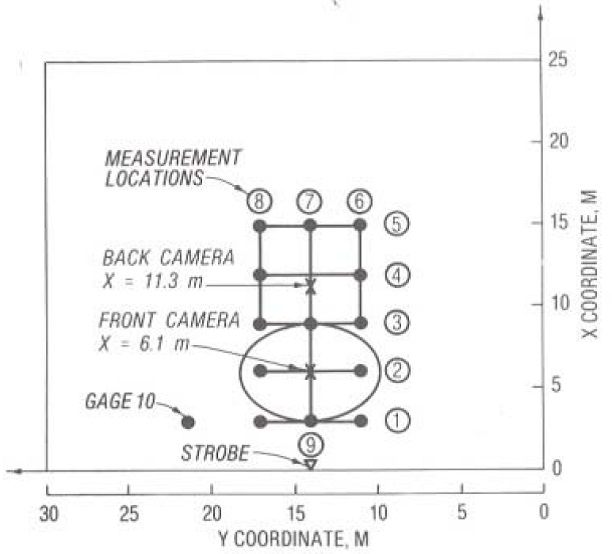
\includegraphics[width=0.4\textwidth]{setup.jpg}
      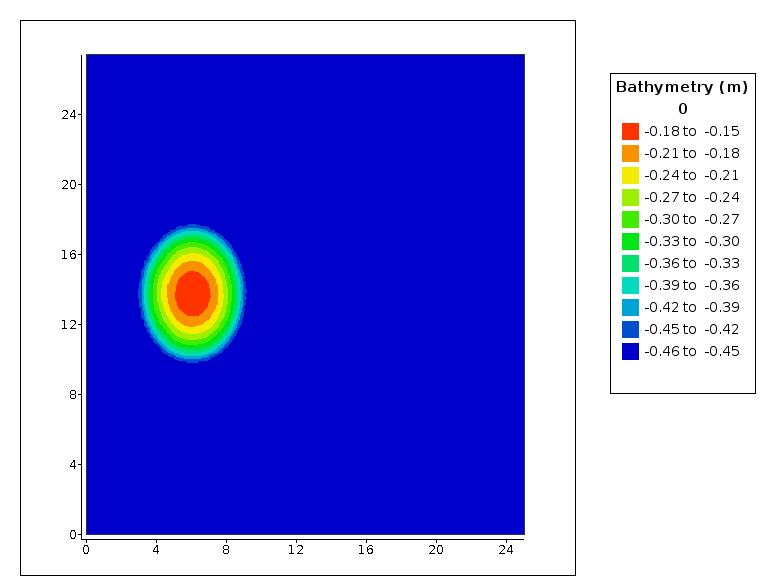
\includegraphics[width=0.55\textwidth]{bathy_shoal.jpg}
      \caption{Set up of Vincent and Briggs experiments}
\end{figure}

Different irregular wave conditions were tested varying the narrowness and the directional spread of the spectrum. They used a TMA shallow-water spectrum (Bouws et al. 1985) and a wrapped normal spreading function which can be close to a Mitsuyasu directionnal spreading function.\\
\begin{table}

\begin{tabular}{|c|c|c|c|c|c|c|c|}
\hline
\hline
Test number (1) & Case ID (2) & Type (3) & Period (sec) (4) & Height (cm) (5) & $\alpha$ (6) & $\gamma$ (7) & $\sigma _m$ (deg) (8) \\
\hline
\multicolumn{8}{|c|}{(a) Initial Series}\\
\hline
1 & M1 & Mono & 1.30 & 5.50 & -- & -- & -- \\
2 & N1 & Spec & 1.30 & 7.75 & 0.01440 & 2 & 10\\
3 & B1 & Spec & 1.30 & 7.75 & 0.01440 & 2 & 30\\
4 & N2 & Spec & 1.30 & 7.75 & 0.00440 & 20 & 10\\
5 & B2 & Spec & 1.30 & 7.75 & 0.00440 & 20 & 30\\
\hline
\end{tabular} \\
\caption{Test conditions for shoal test series, Vincent and Briggs experiments  (1989)}

\end{table}

In this benchmark, only one type of wave condition is tested for the diffraction effects, the N1 one. But B1,B2,N1 and N2 are tested to evaluate the refraction and the shoaling.

\subsubsection{Test-case description}
The case is about spectral wave propagation on a submerged elliptical mound. The study will compare the spectral significant wave heights given by TOMAWAC simulations with measurements from Vincent's experiments.
\paragraph{Geometry of the domain and bathymetry}

\begin{tabular}{ccc}
Bassin & dimension :& 27.43 m * 18.3 m\\
 &depth constant outside the shoal :& 0.4572m\\
Elliptical shoal & major radius :& 3.96m\\
 & minor radius :& 3.05m\\
  & maximum height :& 0.305m\\
  & coordinates of the center :& (6.10,13.72)
\end{tabular}

\vspace{1cm}

The elliptical shoal is defined by :\\
\begin{center}

\begin{tabular}{c|c}
$a = (\frac{x}{3.96})+(\frac{y}{3.05})$ & if $a \geq 1$, $Zf = -0.4572$\\
 & if $a < 1$, $Zf = -0.9144+0.762 \sqrt{1-0.64a}$
\end{tabular}\\
\end{center}
\paragraph{Meshes}
\subparagraph{Spatial discretization}
Three meshes are used for the simulation :
\begin{itemize}
\item finer : Element size at the shoal 0.2m \quad $\Delta x/\lambda$ = 0.09
\item medium : Element size at the shoal 0.4m \quad $\Delta x/\lambda$ = 0.18
\item coarser : Element size at the shoal 0.8m \quad $\Delta x/\lambda$ = 0.35
\end{itemize}

Where $\lambda$ is the wavelenght.
\begin{figure}[h!]
  \centering
    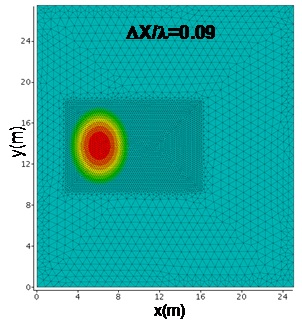
\includegraphics[width=0.3\textwidth]{mesh009.jpg}\\
    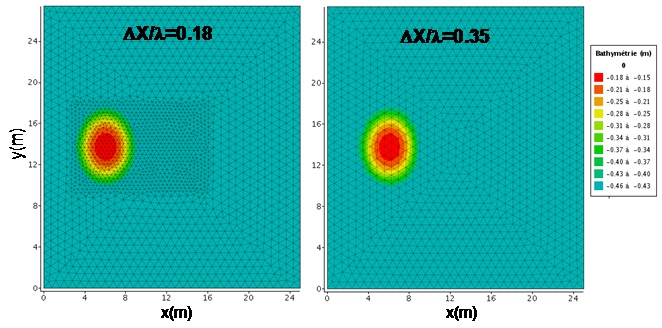
\includegraphics[width=0.65\textwidth]{meshes018035.jpg}
      \caption{The different meshes used}
\end{figure}

\subparagraph{Spectro-angular discretization}
\begin{itemize}
\item 22 frequencies (0.35 - 2.85 Hz)
\item logarithmic scale ($\Delta f/f = 0.1$)
\item 36 directions
\end{itemize}

\paragraph{Initial and Boundary conditions}
The domain is initially at rest.\\
The incident wave conditions are the following :
\begin{itemize}
\item the incident wave conditions are imposed at the boundary representative of the wave generator. All the others are absorbing boundaries.
\item Frequency spectrum : TMA shallow water spectrum
\[S(f,\theta) = E(f)*D(\theta) \]
\[E(f) = \frac{\alpha g^2}{(2\pi)^4}f^{-5} exp(-1.25(\frac{f_p}{f})^{4})*\gamma^{exp(-0.5(\frac{f-f_p}{\sigma f_p})^{2})}*\phi (f,d)
\]
\item Directional spreading function : gaussian type
\[D(\theta) = \frac{1}{\sqrt{2\pi}\sigma _m}exp[-\frac{(\theta - \theta _m)^2}{2\sigma^2_m}]
\]
\end{itemize}
Where :\\
\begin{itemize}
\item $\alpha$ : Phillips constant
\item $f_p$ : peak frequency ($f_p = 0.769$ Hz)
\item $\gamma $: peak factor
\item $\sigma = \left\{ \begin{array}{rl}
 0.07 &\mbox{ if $f<f_p$} \\
  0.09 &\mbox{ if $f>f_p$}
       \end{array} \right.$
\item $\phi (f,d)$ is a factor which allows the consideration of depth effects :\\
$\phi (f,d) = \left\{ \begin{array}{rl}
 0.5 w^2_p &\mbox{ if $w_d\le 1$} \\
  1-0.5(2-w_d)^2 &\mbox{ if $1<w_d<2$}\\
  1 &\mbox{ if $2 \le w_d$} \\
       \end{array} \right.$\\
       with $w_d = 2\pi f(d/g)^{1/2}$
       \item$\theta _m$ : mean wave direction at frequency f
       \item $\sigma _m$ : directional spreading parameter
\end{itemize}
\begin{figure}[h!]
  \centering
    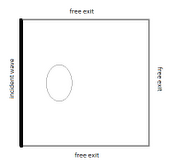
\includegraphics[width=0.5\textwidth]{boundary_limit.png}
      \caption{The boundary conditions}
\end{figure}

\subsubsection{Numerical parameters}
\begin{itemize}
\item time steps :
	\begin{enumerate}
    \item $\Delta x / \lambda = 0.09  \rightarrow \Delta t = 0.005 $
    \item $\Delta x / \lambda = 0.18  \rightarrow \Delta t = 0.025 $
    \item $\Delta x / \lambda = 0.35  \rightarrow \Delta t = 0.1 $
  \end{enumerate}
\item CPU times : \\
\begin{tabular}{cccc}
 & $\Delta x / \lambda = 0.09 $ &$\Delta x / \lambda = 0.18 $&$\Delta x / \lambda = 0.35 $\\
 B1 & -- & 1569 s & 209 s \\
 B2 & -- & 1387 s & 211 s \\
 N2 & -- & 1534 s & 239 s \\
 N1 & 4027 s & 1359 s & 229 s\\

\end{tabular}
\end{itemize}

\subsubsection{TOMAWAC Results }
At first, simulations without diffraction effects are done in order to validate the propagation and refraction of the wave over this complex bathymetry. To compare the simulation results and the measurements of Vincent and Briggs (1989), the significant wave heights have been normalized by the incident significant wave height.\\
\begin{itemize}
\item B1 and B2 tests (wide directional spreading):\\
A good matching can be see in these tests (see Figure 5). After drawing the iso-wave-height compared to the Vincent's measurements, the wave concentration zone is well represented. The amplification factor goes over 1.3 for B1 and 1.4 for B2. As in measurements, this amplification factor is a bit higher for B2 case (higher peak factor) than for B1 case. But simulation factors are little bit higher than those measured.\\
Moreover, the computations of normalized wave height along the transect 4 match quite well with the measurements (not shown here).\\
\begin{figure}[H]
  \centering
  \begin{tabular}{cc}
  	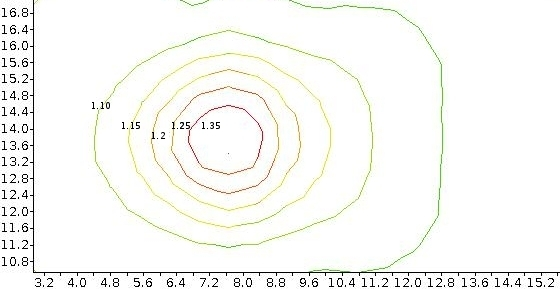
\includegraphics[width=0.4\textwidth]{iso-B1.jpg}&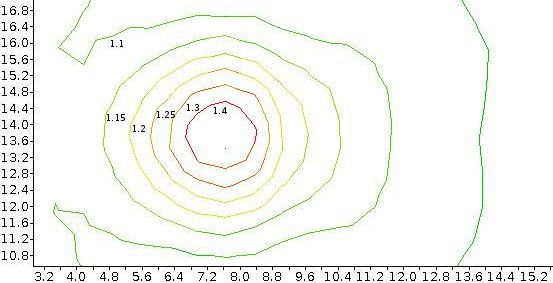
\includegraphics[width=0.4\textwidth]{iso-B2.jpg}\\
  	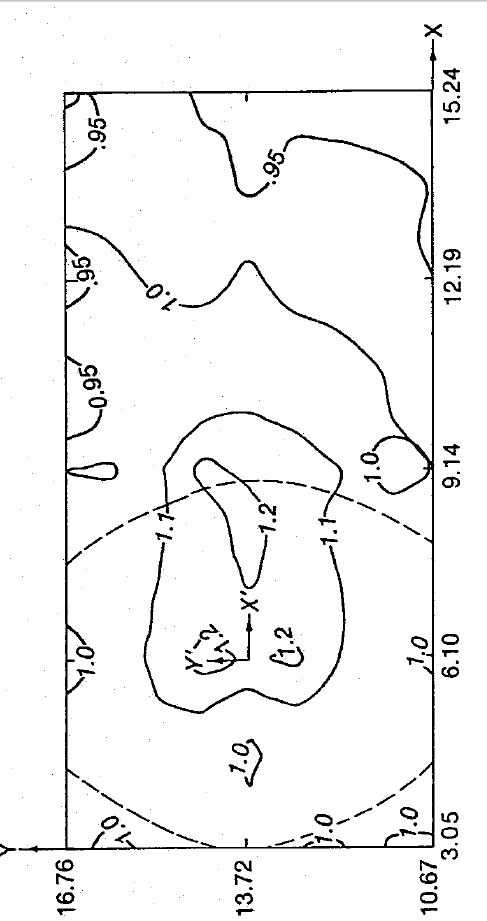
\includegraphics[width=0.22\textwidth,angle=-90]{B1_m.JPG}
 	&
    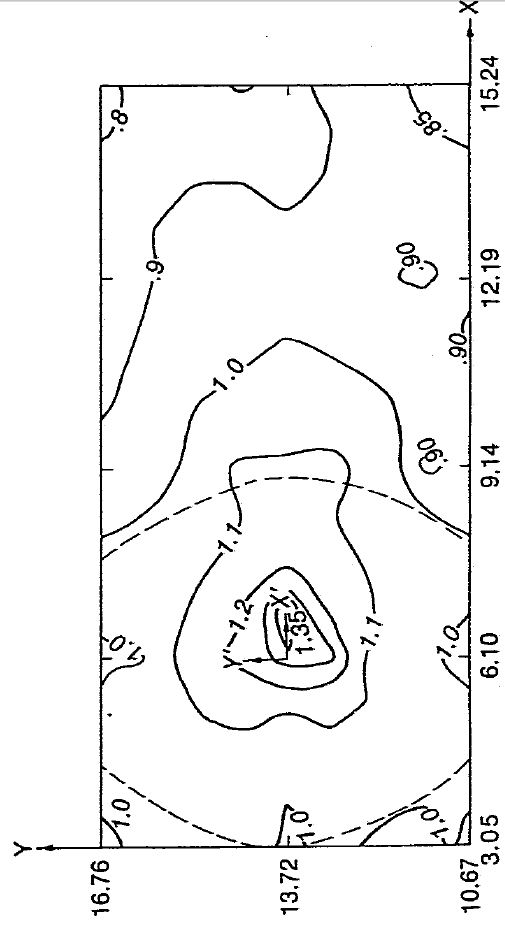
\includegraphics[width=0.21\textwidth,angle=-90]{B2_m.JPG}\\
     \end{tabular}
      \caption{Comparaison of normalized significant wave height iso-lines for the B1 (left) and B2 (right) tests with the measurements from Vincent and Briggs.(coarser mesh).}
\end{figure}

\item N1 and N2 tests (narrow directional spreading):\\
These tests are not as good as the B ones because only one area of big wave heights is shown while two are highlighted in measurements. Also the amplificator factors are bigger than those measured. It can be explain by the lack of representation of the diffraction effects. But again, the results along the transect 4 show a coherence of the simulation and the measurements. (see Figure 6, see Figure 7 and 8 for N1).
\begin{figure}[H]
  \centering
    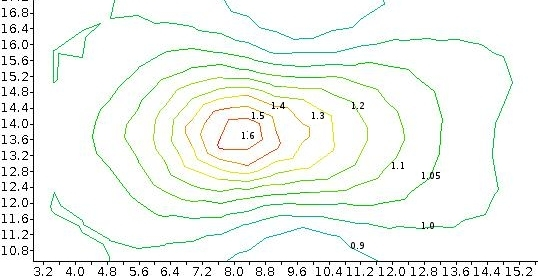
\includegraphics[width=0.5\textwidth]{iso-N2.jpg}
    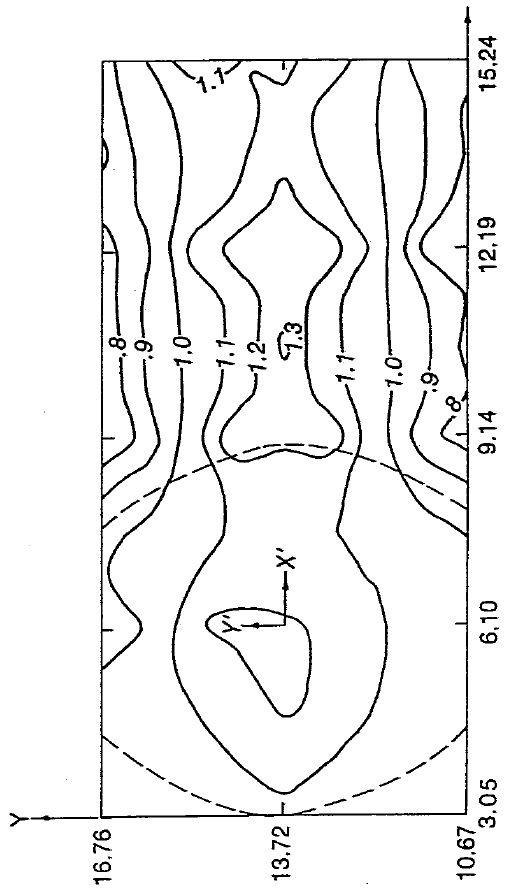
\includegraphics[width=0.3\textwidth,angle=-90]{N2-m.JPG}
      \caption{Comparaison between normalised iso-line TOMAWAC results and Vincent measurements for the case N2 (coarser mesh). }
\end{figure}
\end{itemize}
Subsequently, the computation will include diffraction effects.
The diffraction coefficient $K_d$ is defined by the ratio of the spectral significant wave height to the spectral significant incident wave height, $K_d = \frac{H_{m0}}{H_{m0\_ inc}}$.\\
Parametrical tests have shown the influence of two non-dimensional parameters : the ratio of the mesh size over the wavelength ($\Delta x / \lambda$) and the current number.
The courant number Cr is : $Cr = \frac{C_g(f_p)\Delta t}{\Delta x}$.\\
where $C_g(f_p)$ is the group velocity associated to the sea-state peak frequency, $\Delta t$ the simulation time step and $\Delta x$ the size of the smallest element of the mesh.\\ 
The diffraction coefficients obtained during the simulations (changing Cr and $\Delta x / \lambda $) are compared with Vincent and Briggs measurements and the iso-Kd curves resulting from TOMAWAC simulations are superposed with the ones measured by Vincent and Briggs. (see Figure 8). 


\begin{figure}[!h]
  \centering
    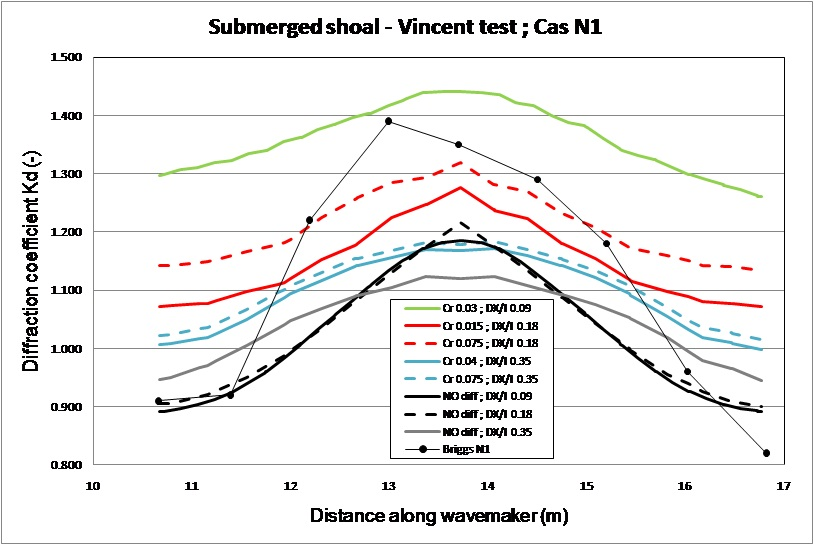
\includegraphics[width=0.85\textwidth]{Kd.jpg}
      \caption{Comparaison between TOMAWAC results and Vincent measurements: measured and simulated values of the diffraction coefficient along the transect 4 \textit{(see Figure 1)} of the model}
\end{figure}
\begin{figure}[H]
  \centering
\begin{tabular}{cc}
    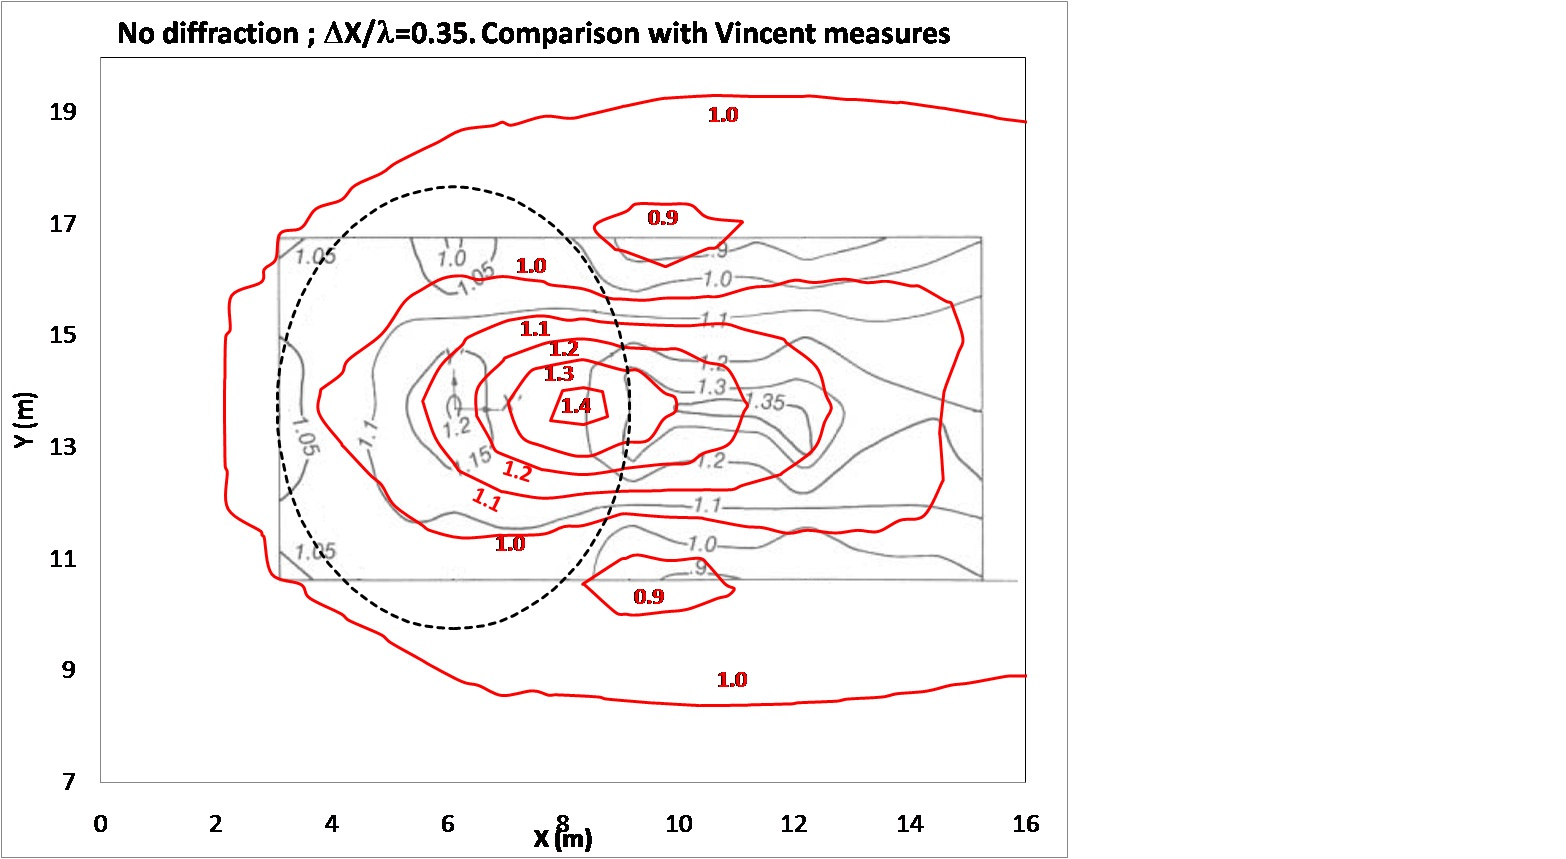
\includegraphics[width=0.65\textwidth]{iso-Kd_nodiff_dx035.jpg}& \hspace{-3cm}
    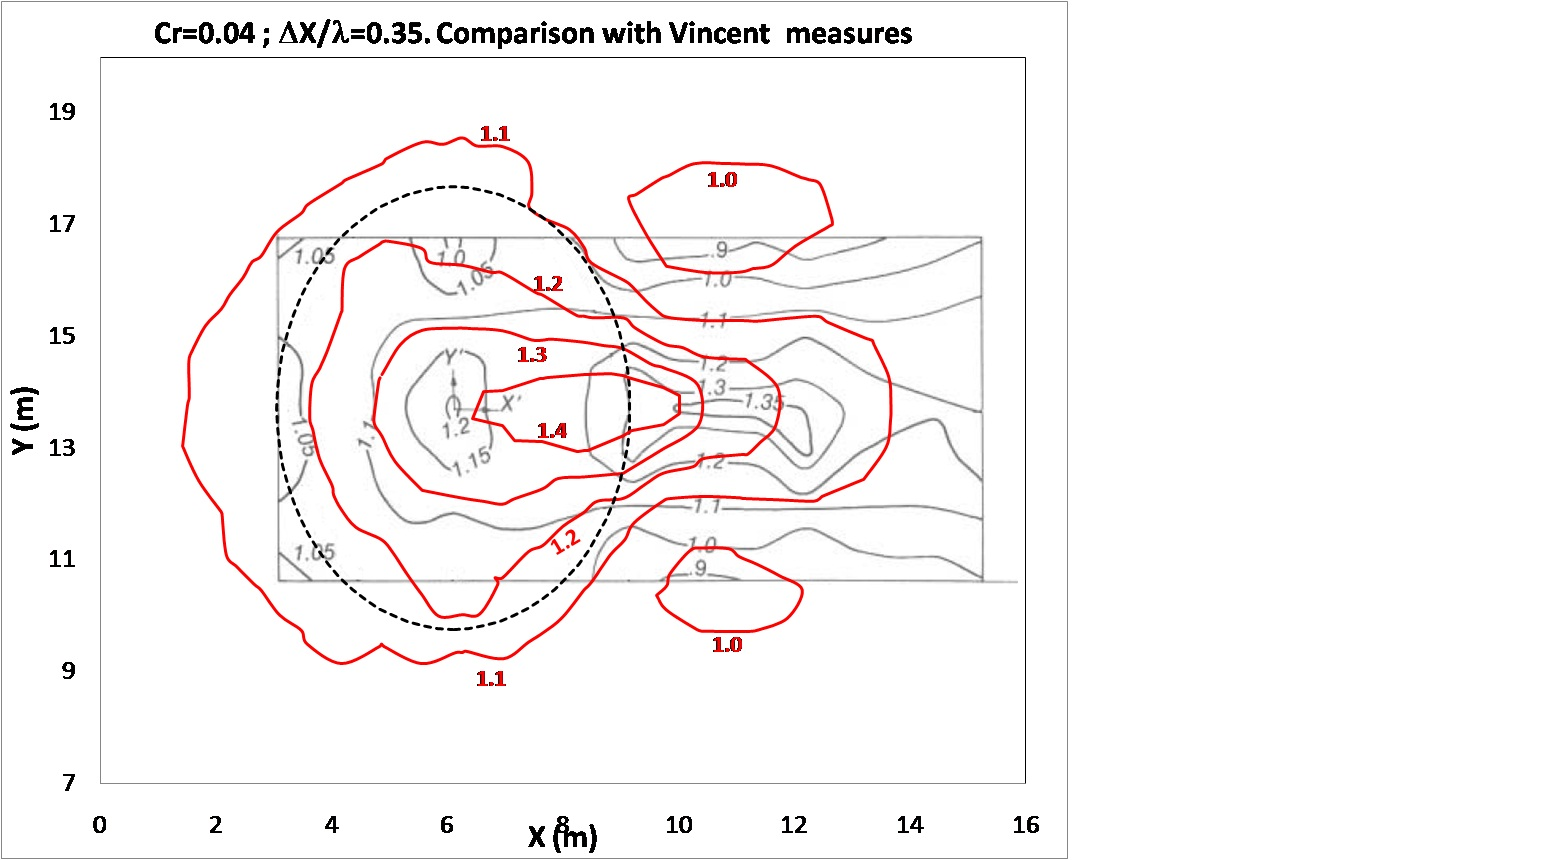
\includegraphics[width=0.65\textwidth]{iso-Kd_cr004-dx035.jpg}\\
    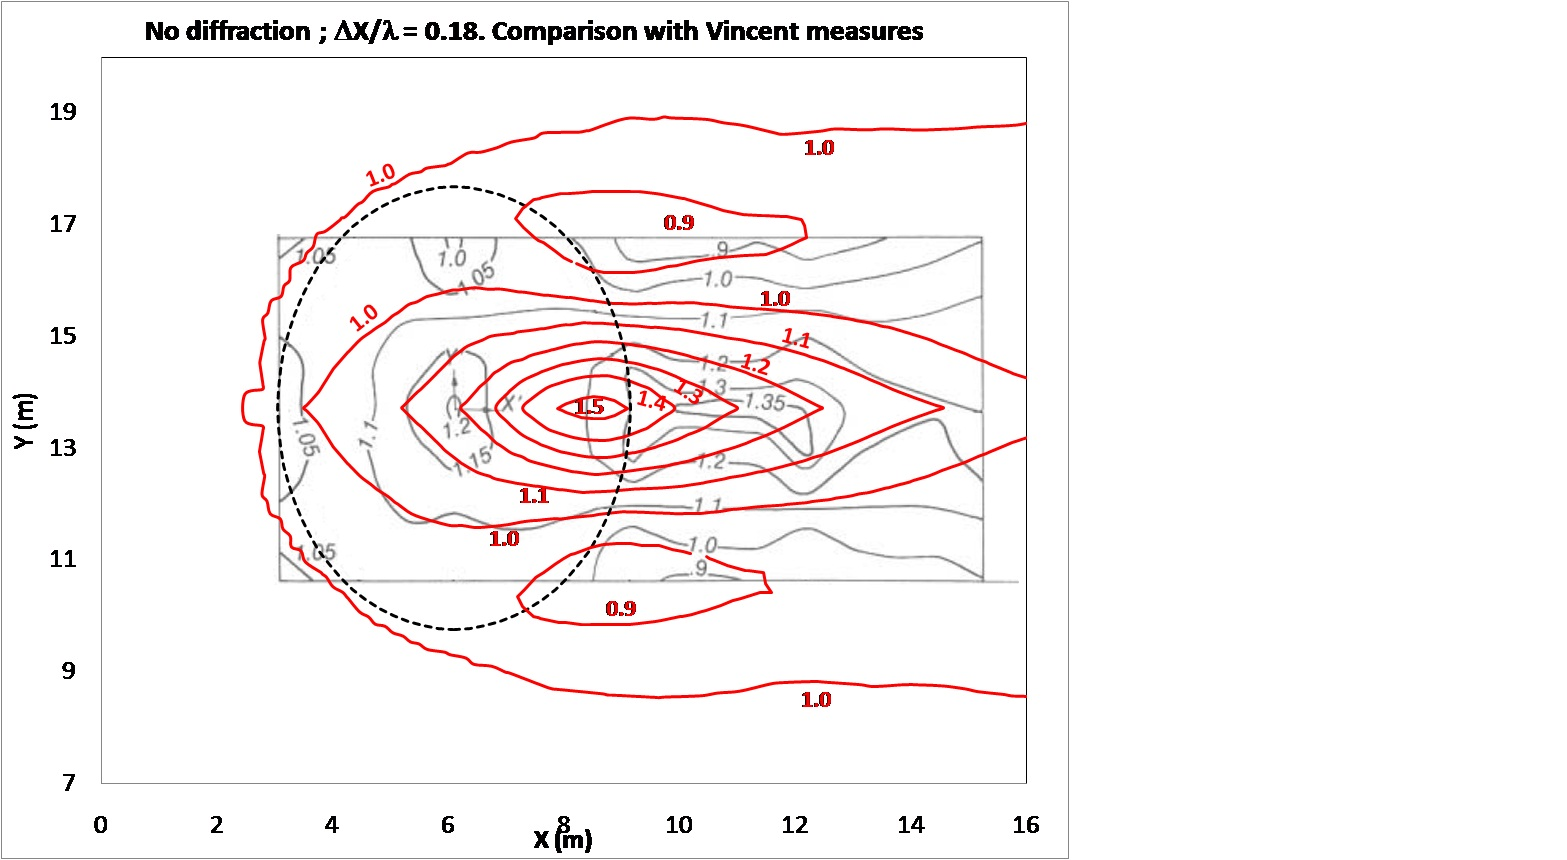
\includegraphics[width=0.65\textwidth]{iso-Kd_nodiff_dx018.jpg}& \hspace{-3cm}
    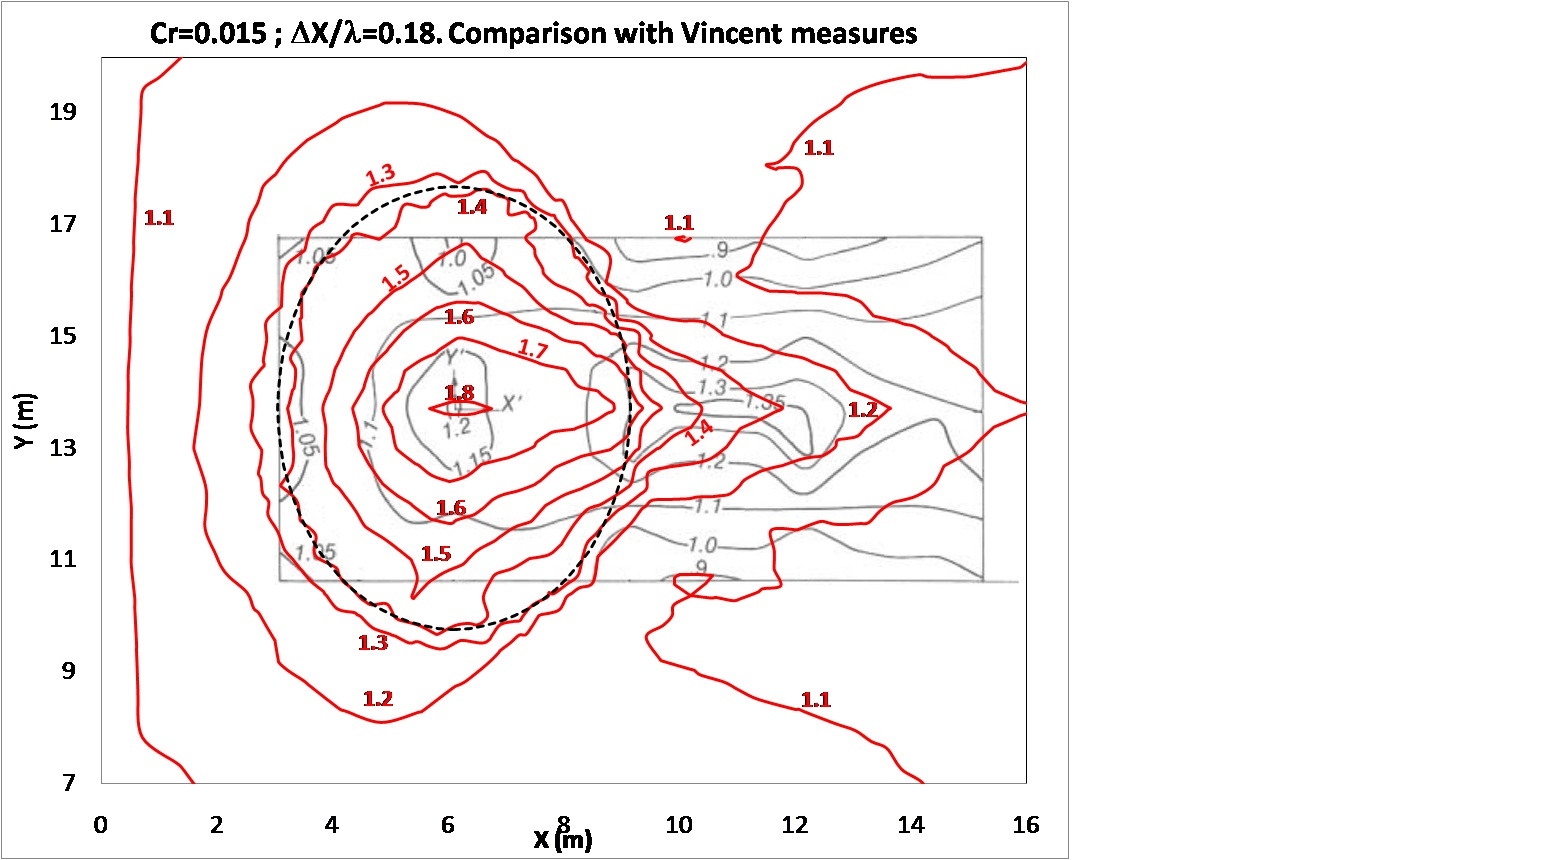
\includegraphics[width=0.65\textwidth]{iso-Kd_cr0015_dx018.jpg}\\
    \end{tabular}

      \caption{Comparaison between TOMAWAC results and Vincent measurements: measured and simulated iso-Kd curves over and behind the mound for the case N1}
\end{figure}


As can bee seen in these two graphs (Figures 7 \& 8), the diffraction effects over the shoal are not well simulated by TOMAWAC due to a large build-up of energy. Indeed the larger Cr is and the finer the mesh is, the larger the numerical and the energy build-up are. Moreover with the coarser mesh ($\Delta x / \lambda = 0.35$) TOMAWAC is not able to capture the diffraction effects generated by the submerged shoal. In the Figure 6, the simulation's curves are too flattened and the curves taht have the shape closest to the measurements are the No diffraction ones. Also in the iso-Kd graph, the curves do not superimpose well when diffraction is taken into account, but for the case with only propagation and refraction the correspondance is correct. Indeed, we can see that the iso-line shapes are closest to the measured ones.\\
Mainly, the build-up and the numerical noise are generated when a high resolution of the mesh is used and they are due to the meshfree algorithm (used to compute second derivatives during simulation). 
In order to improve the simulation of the diffraction effects, a spatial filter is built to limit the energy build-up. The effect of this filter can be seen on the diffraction coefficient Kd (see Figure 9). The noise and the enrgy build-up effects are reduced but it does not improve the quality of the results significantly.\\

\begin{figure}[H]
  \centering
    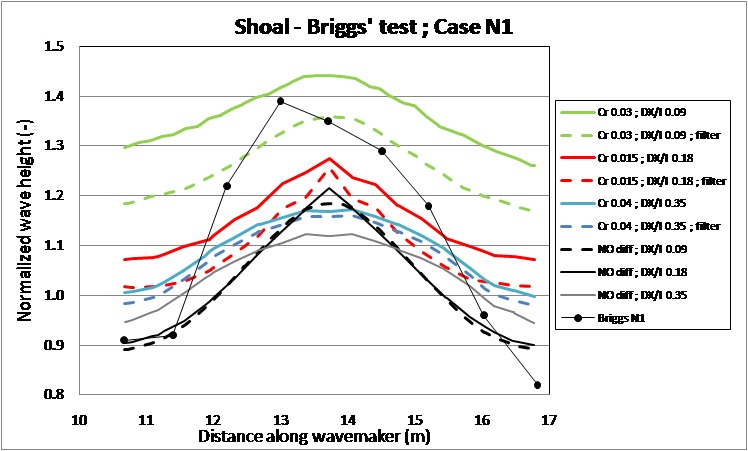
\includegraphics[width=0.85\textwidth]{kd_filter.jpg}
      \caption{Comparaison between TOMAWAC results and Vincent measurements: measured and simulated values using a filter of the diffraction coefficient along the transect 4 of the model}
\end{figure}

\subsubsection{Conclusion}
This benchmark test allows to compare simulations from TOMAWAC and experimental results. It follows that TOMAWAC provides a correct simulation of the propagation, shoaling and the refraction but the diffraction effects are limited and not really well represented. In order to improve the results, a smoothing filter can be applied on the spatial domain.\\

\subsubsection*{Rerences}
\bibliography{b}
 VINCENT C.L.,BRIGGS M.J. (1989) : Refraction-diffraction of irregular waves over a mound. \textit{Journal os Waterway, Port,Coastal and Ocean Engineering, Vol.115, N2, pp 269-284}\\
 MATTAROLO G. (2012) : Simulating diffraction in the third generation spectral model TOMAWAC. Implementation and testing of a model based on previous research work. \textit{H-P74-2012-00439-EN, pp19-48}\\
 F. BECQ, M. BENOIT (1996) : Fiche cas-test : Propagation de houle sur un haut fond elliptique. \textit{Extrait de la note HE-42/96/010/B Logiciel TOMAWAC de modelisation des tats de mer en elements finis, Dossier de validation de la version 1.0} 
